\newpage
\chapter{Nombres Complexes}
\vspace{3mm} %5mm vertical space
\section{Conversion polaire - cartésienne}
\vspace{3mm} %5mm vertical space

Définition du module: \\

le module noté $|Z|$ est la longueur du segment (rayon). Elle peut être mesurée  grâce à la formule de pythagore ($\sqrt{a²+b²}$). \\


\vspace{5mm} %5mm vertical space
Représentation Géographique \\

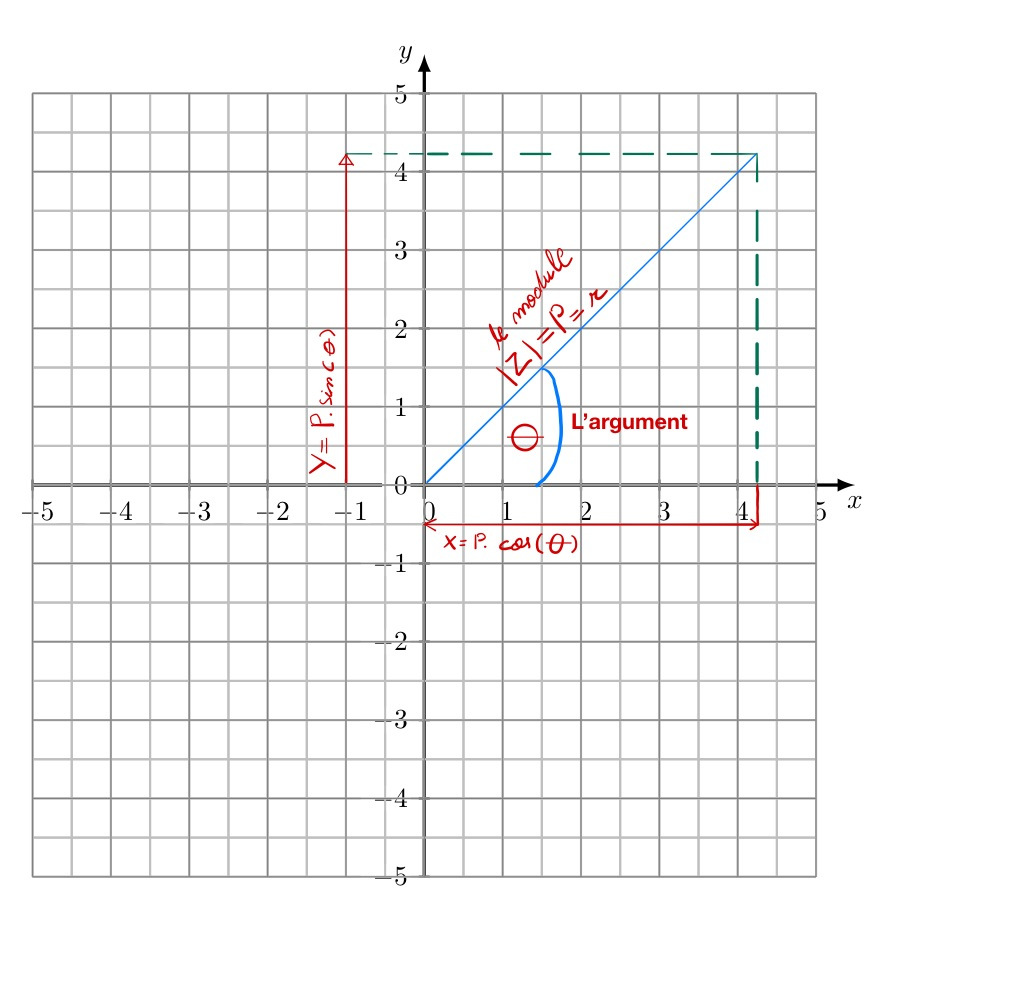
\includegraphics[scale=1.5]{cart-mod}
\vspace{2mm} %5mm vertical space

Démonstration : \\

$|Z| = \rho cos(\theta)+ \rho sin(\theta) *i$ \\
$|Z| = \sqrt(\rho^{2} cos(\theta)^{2}+ \rho^{2} sin(\theta)^{2})$ \\
$|Z| = \sqrt(\rho^{2} cos(\theta)^{2}+ sin(\theta))*i $ \\
$|Z| = \sqrt(\rho^{2}) $ \\
$|Z| = \rho $ \\

$\rho$ est le module et $\theta$ est l'argument \\
$Z= P(cos(\theta) + sin(\theta)*i )$ ou $Z= P(cis(\theta))$\\

\newpage

\section{Conversion Cartésienne - Polaire}
\vspace{3mm} %5mm vertical space

$\rho$ = $\sqrt(x²+y²)$ \\

Démonstration Géométriquement $\theta$ \\

Nous pouvons voir que $\theta$ est modifié en fonction de X et de Y que si nous dessinons un cercle, nous pouvons voir que le segment Y est une tangeante au cercle de rayon X. \\

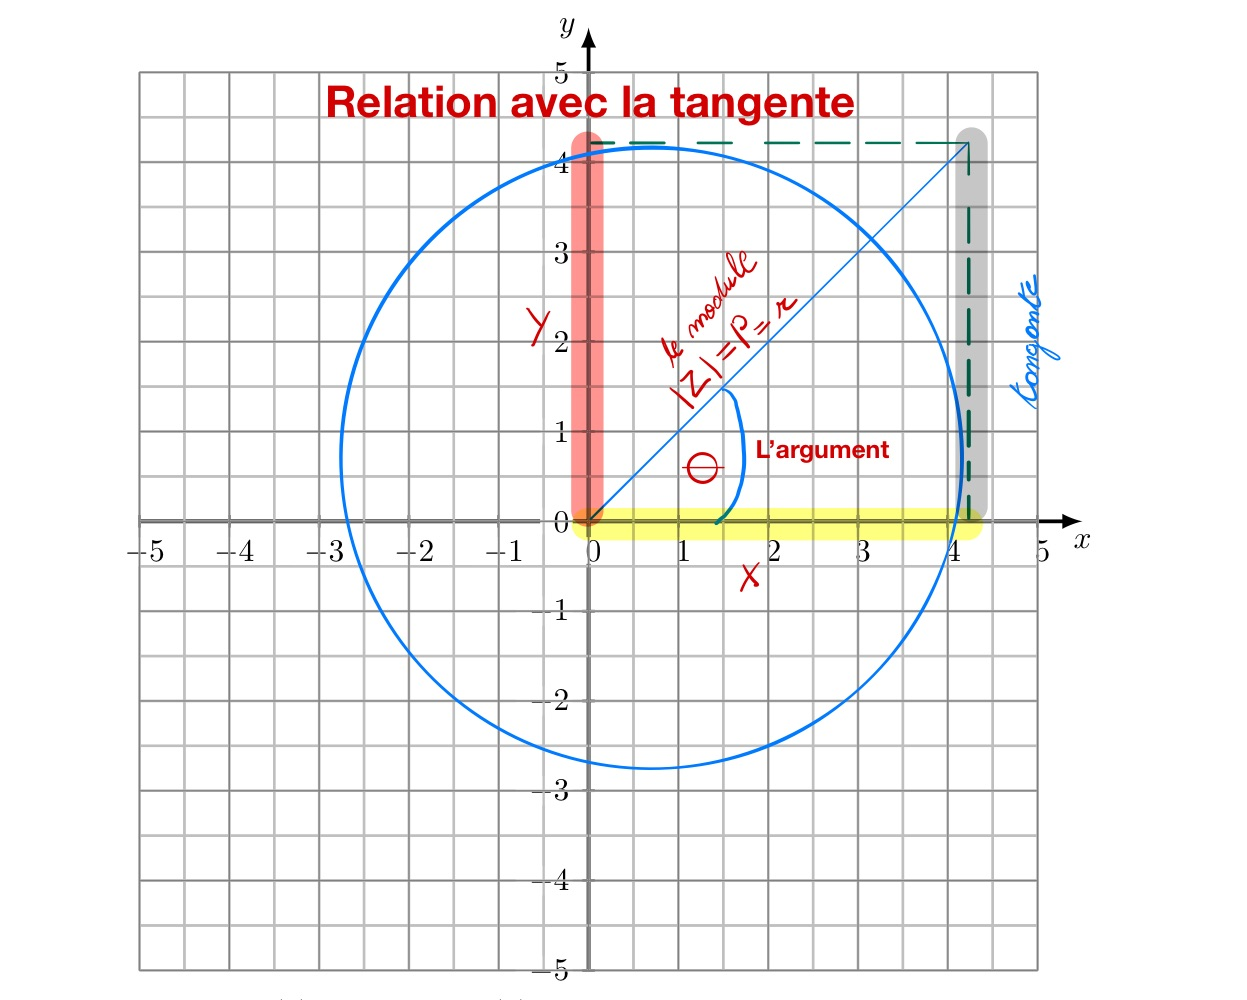
\includegraphics[scale=0.3]{cart-tg}

$X=\rho * cos(\theta)$ $ $ $ Y=\rho * sin(\theta)$

\vspace{5mm} %5mm vertical space
Démonstration Algébriquement $\theta$ \\

$\frac{Y}{X}$ = $\frac{\rho * sin(\theta)}{\rho * cos(\theta)}$ \\
$\frac{Y}{X}$ = $\frac{sin(\theta)}{cos(\theta)}$ \\
$\frac{Y}{X}$ = tg($\theta)$ \\

\vspace{5mm} %5mm vertical space
Conclusion : \\

$\theta = arctg(\frac{Y}{X})$ \\

$tg(\theta) = \frac{Y}{X}$


\newpage

\section{Conversion exponentielle - cartésienne}
\vspace{3mm} %5mm vertical space



\newpage
\section{Nombre Complexes addition}
\vspace{3mm} %5mm vertical space

$(4 * cis(45^{\circ} )) + (5 * cis(\frac{\pi}{3}))$

\vspace{10mm}
\textbf{Calcul du module}
\vspace{5mm}

$\rho = \sqrt{\rho_{1}^{2} + \rho_{2}^{2} + \rho_{1} \rho_{2} cos(\theta_{1} - \theta_{2}) }$ \\

$\rho = \sqrt{4^{2} + 5^{2} + 2 * 4 * 5 cos(45^{\circ} - 60^{\circ})}$ \\

$\rho = \sqrt{41 + 40 * 0,96592582628}$ \\

$\rho = \sqrt{79,6370330512}$ \\

$\rho = 8,923958373457376 $ \\

\vspace{6mm}
\textbf{Calcul de l'argument}
\vspace{5mm}

$\theta = arctg(\frac{\rho_{1}sin(\theta_{1}) + \rho_{2}sin(\theta_{2})} {\rho_{1}cos(\theta_{1}) + \rho_{2}cos(\theta_{2})} )$ \\

$\theta = arctg(\frac{4sin(45^{\circ}) + 5sin(60^{\circ})} {4cos(45^{\circ}) + 5cos(60^{\circ})} )$ \\

$\theta = arctg(\frac{4\frac{\sqrt{2}}{2}) + 5\frac{\sqrt{3}}{2} } {4\frac{\sqrt{2}}{2}) + 5\frac{1}{2}})$ \\

$\theta = arctg(1.3434647741399612)$ \\

$\theta = arctg(53.3380661^{\circ})$ \\

\vspace{6mm}
\textbf{Solution}
\vspace{5mm}

$|Z| = 8,923 cis(53.338^{\circ})$

\newpage
\section{Nombre Complexes soustraction}
\vspace{3mm} %5mm vertical space

\newpage
\section{Nombre Complexes multiplication}
\vspace{3mm} %5mm vertical space

% (b) (4 × cis(45 ◦ )) × (5 × cis( π 3 ))


\newpage
\section{Nombre Complexes division}
\vspace{3mm} %5mm vertical space
